\chapter{Background}

\section{Automatic Identification Systems (AIS)}

As already mentioned in \cref{sec:topics_covered}, \acrfull{ais} was initiated by \acrfull{imo} and since 2004 every commercial and passenger vessel exceeding 299 \acrfull{gt} is required to carry an \acrshort{ais} transmitter. These transmitters broadcasts \acrshort{ais} messages following the \gls{aivdm} protocol. The \gls{aivdm} protocol contains two main types of reports: positional and static. The positional reports contains automatically collected information such as the transmitting vessel's \acrfull{mmsi} number, the current timestamp, and the vessel's current navigational data including the current geographical coordinates, \acrfull{sog}, \acrfull{cog}, true heading, \acrfull{rot}, and more. The static reports contain additional information about the vessel and its current voyage, some of which are manually inputted, such as the vessel's \acrshort{imo} number, name, dimensions, draft, intended destination and \acrfull{eta}.

Regarding vessel identification there are mainly two values that are unique to a given vessel: the \acrshort{mmsi} and \acrshort{imo} numbers. Both of these should be unique on its own to a certain vessel, however, \acrshort{mmsi} numbers can be recycled under certain conditions such as when a vessel is put out of commission while the \acrshort{imo} number is specific to a vessel's hull. Therefore, \acrshort{imo} is the preferred identifier, however, since the \gls{aivdm} protocol divides these identifiers in positional and static reports, both needs to be considered in order to use both static and positional \acrshort{ais} information.


\section{Vessel segmentation and additional information}

% \begin{figure}[htbp]  % order of priority: h here, t top, b bottom, p page
%     \centering
%     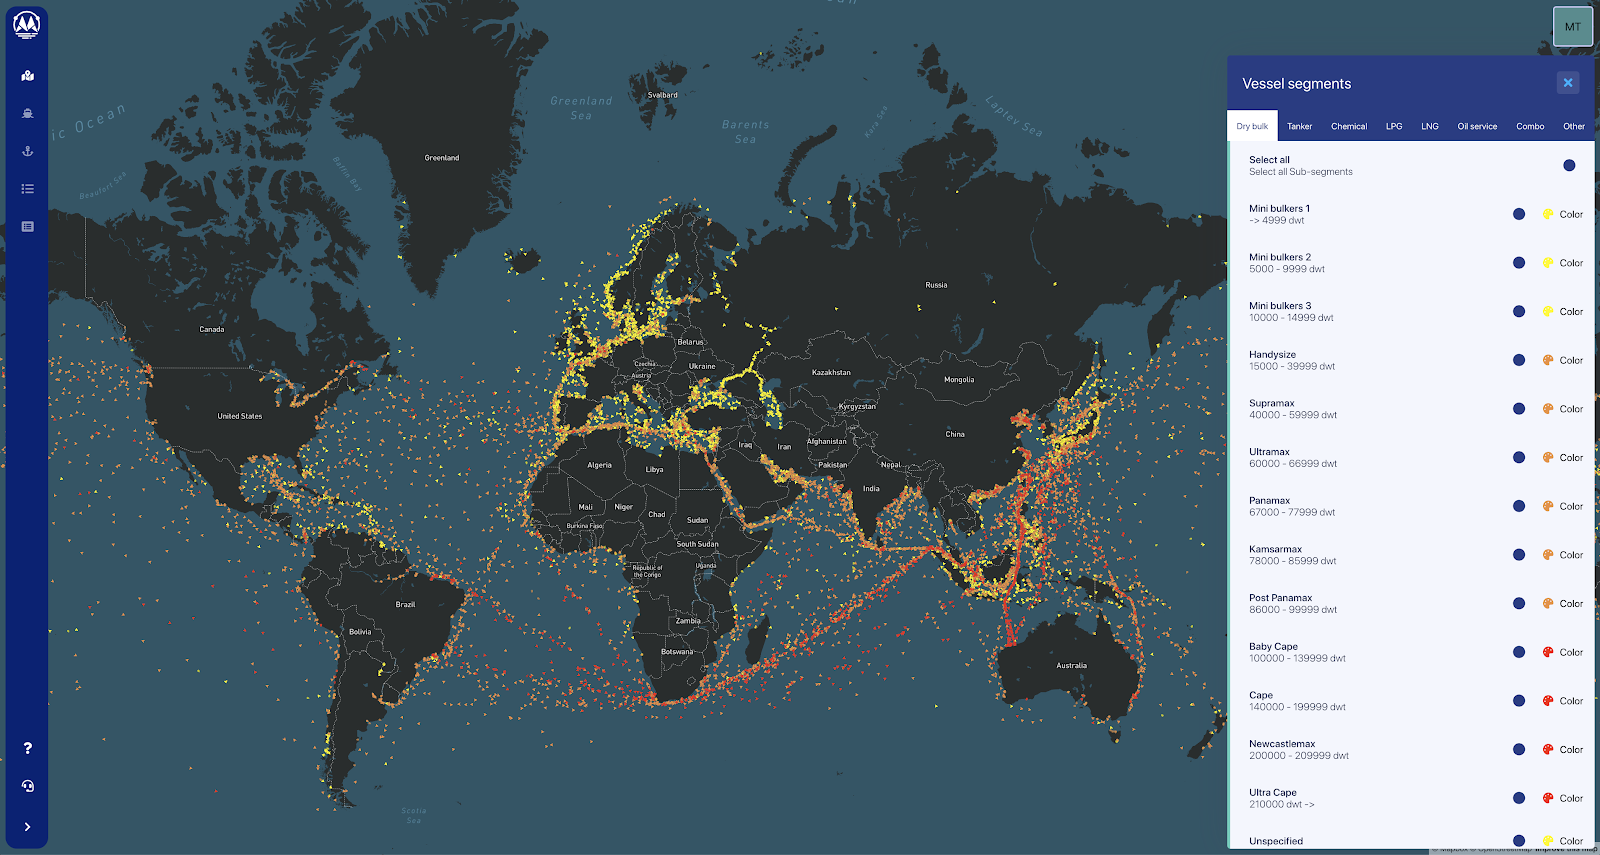
\includegraphics[width=.89\textwidth]{figures/segment_map}
%     \caption{Maritime Optima’s segmentation of vessels where yellow vessels are smaller than reds}
%     \label{fig:segment_map}
% \end{figure}
%
% The collaborative company Maritime Optima AS has implemented a method of dividing vessels into segments and subsegments (categories and sub-categories). \cref{fig:segment_map} shows the differences in route patterns between different sub-segments (colored from yellow to red relevant to the dimensions of the vessels) for dry cargo vessels. Considering this information in the prediction methods can be a novel approach to the problem area. Maritime Optima has also expressed the novelty of this problem area through thorough competitor analysis and claims that providing accurate predictions is of high value for their customers is a factor that can improve their decision making and investments.

\section{Machine learning (ML)}

\section{}
